\section{Problem 3}
\begin{frame}
        \frametitle{Problem 3(a) – Setup}

    \begin{figure}
        \centering
        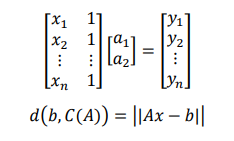
\includegraphics[height = 0.5\textheight]{img/setup3_1.png}
    \end{figure}

    \end{frame}

\begin{frame}[fragile] 
    \frametitle{Problem 3(a) – Code}
    % 代码块参数:语言,标题
    % 请减少代码初始的缩进
    \begin{codeblock}{c++}{C++代码}
        //ATAx = ATb
        F_result = (A.transpose() * A).ldlt().solve(A.transpose() * b);
        cout << "The solution using normal equations is:\n"

            << F_result << endl;
        //输出距离
        norm = (A * F_result - b).norm();
        cout << "The distance is :\n"
            << norm << endl;
    \end{codeblock}
    % \begin{figure}
    %     \centering
    %     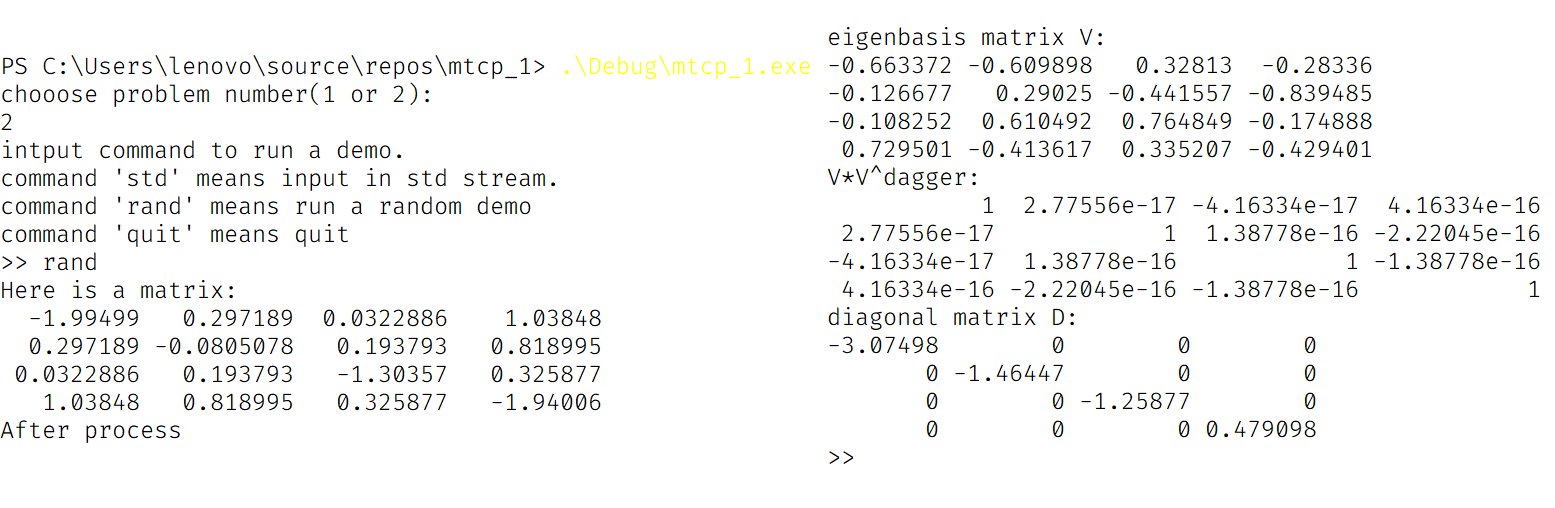
\includegraphics[height = 0.8\textheight]{img/result2.png}
    % \end{figure}
\end{frame}

\begin{frame}         % 注意添加 fragile 标记
    \frametitle{Problem 3(a) – result}

    \begin{figure}
        \centering
        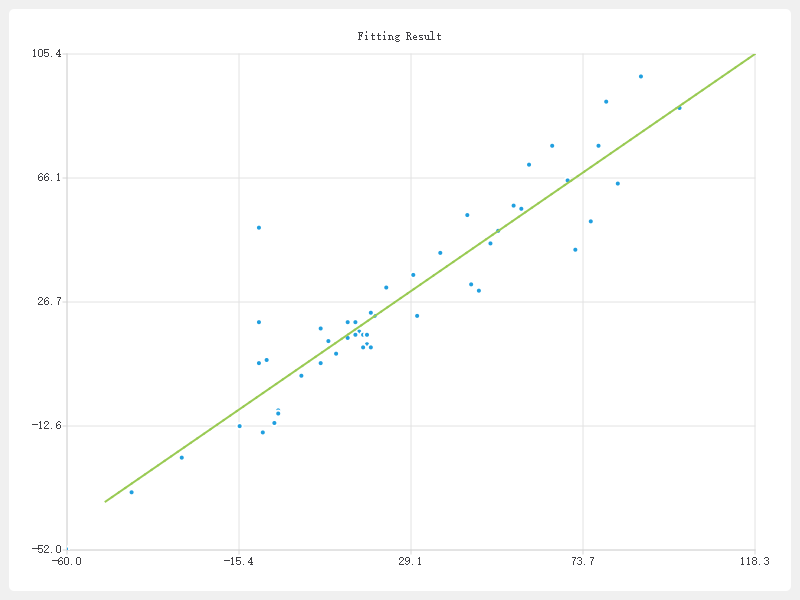
\includegraphics[height = 0.5\textheight]{img/result3_1.png}
    \end{figure}
        \begin{equation}
        d(b,C(A))=84.89
    \end{equation}
\end{frame}
\begin{frame}
        \frametitle{Problem 3(b) – Setup}

    \begin{figure}
        \centering
        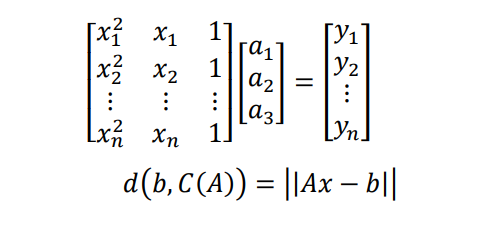
\includegraphics[height = 0.5\textheight]{img/setup3_2.png}
    \end{figure}

    \end{frame}
\begin{frame}[fragile] 
    \frametitle{Problem 3(b) – Code}
    % 代码块参数:语言,标题
    % 请减少代码初始的缩进
    \begin{codeblock}{c++}{C++代码}
        for (int i = 0; i < N; i++) {
            A(i, 0) = mat(i, 0);
            A(i, 1) = mat(i, 0) * mat(i, 0);
            A(i, 1) = 1;
            b(i) = mat(i, 1);
        }
        //ATAx = ATb
        F_result = (A.transpose() * A).ldlt().solve(A.transpose() * b);
        cout << "The solution using normal equations is:\n"

            << F_result << endl;
        //输出距离
        norm = (A * F_result - b).norm();
        cout << "The distance is :\n"
            << norm << endl;
    \end{codeblock}
    % \begin{figure}
    %     \centering
    %     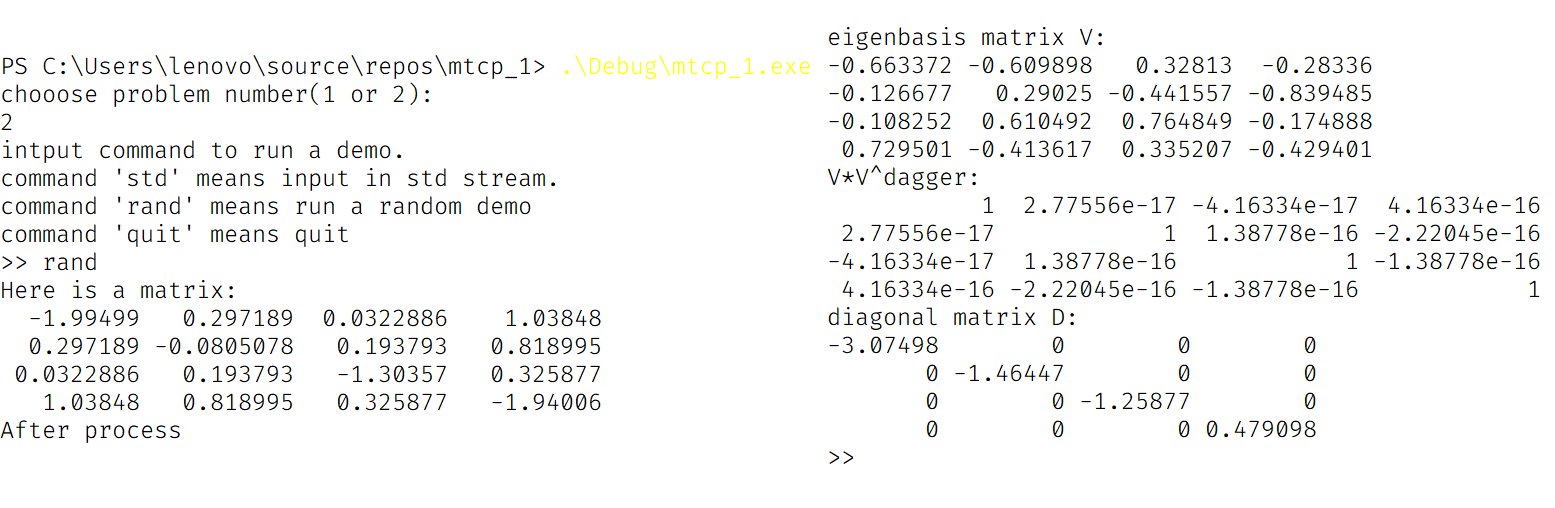
\includegraphics[height = 0.8\textheight]{img/result2.png}
    % \end{figure}
\end{frame}

\begin{frame}         % 注意添加 fragile 标记
    \frametitle{Problem 3(b) – result}

    \begin{figure}
        \centering
        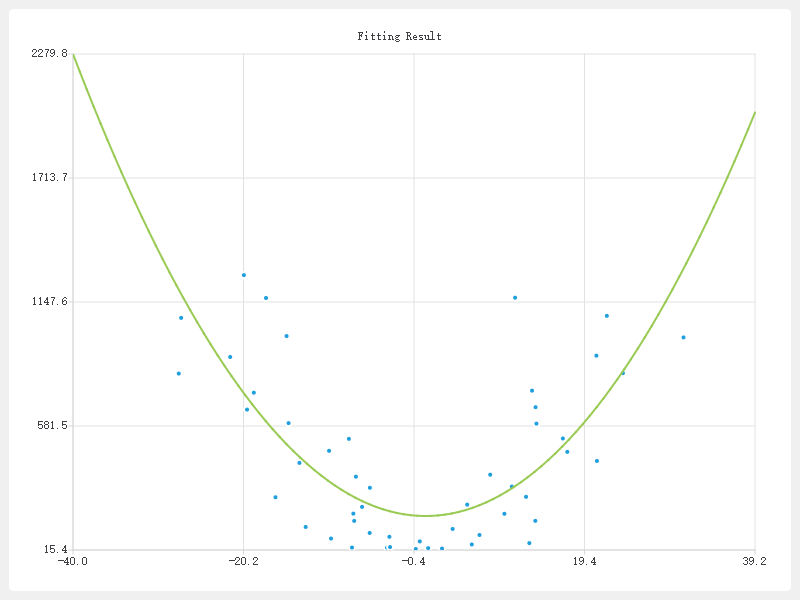
\includegraphics[height = 0.5\textheight]{img/result3_2.png}
    \end{figure}
        \begin{equation}
        d(b,C(A))=1789.58
    \end{equation}
\end{frame}
